\par Voici à très haut niveau les grandes étapes de cet essai:
\label{methodologie_haut_niveau}
\begin{figure}[H]
    \centering
    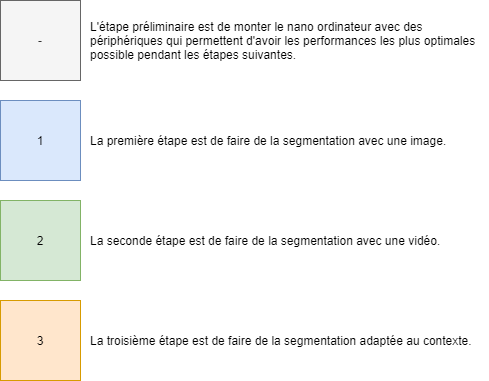
\includegraphics[width=0.75\textwidth]{methodologie_haut_niveau}
    \caption{Organigrame de la méthodologie à haut niveau}
    \label{fig:methodologie_haut_niveau}
\end{figure}
\par Pour y parvenir, la méthodologie suivante a été suivie et permet d'évaluer les performances de base de la segmentation sémantique avec le nano ordinateur.
\label{methodologie_simple}
\begin{figure}[H]
    \centering
    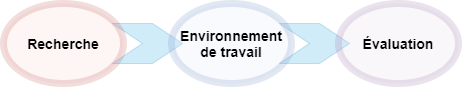
\includegraphics[width=0.65\textwidth]{methodologie_simple}
    \caption{Organigrame de la méthodologie pour évaluer les performances}
    \label{fig:methodologie_simple}
\end{figure}
\par Si chacun des blocs est explosé, chacun d'eux s'organise autour des activités suivantes: 
\label{methodologie_simple_details}
\begin{figure}[H]
    \centering
    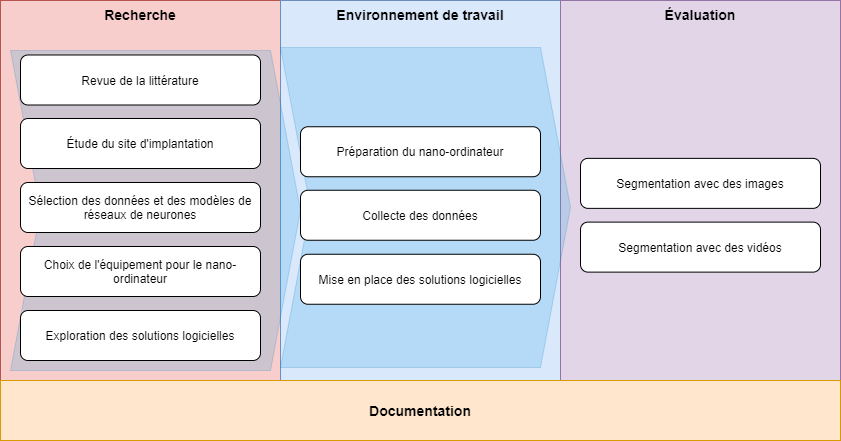
\includegraphics[width=1.0\textwidth]{methodologie_simple_details}
    \caption{Organigramme des détails de la méthodologie pour évaluer les performances}
    \label{fig:methodologie_simple_details}
\end{figure}
\par Si l'évaluation est probante, la méthodologie se verra bonifiée par des étapes d'adaptation et de traitement. 
\label{methodologie_complexe}
\begin{figure}[H]
    \centering
    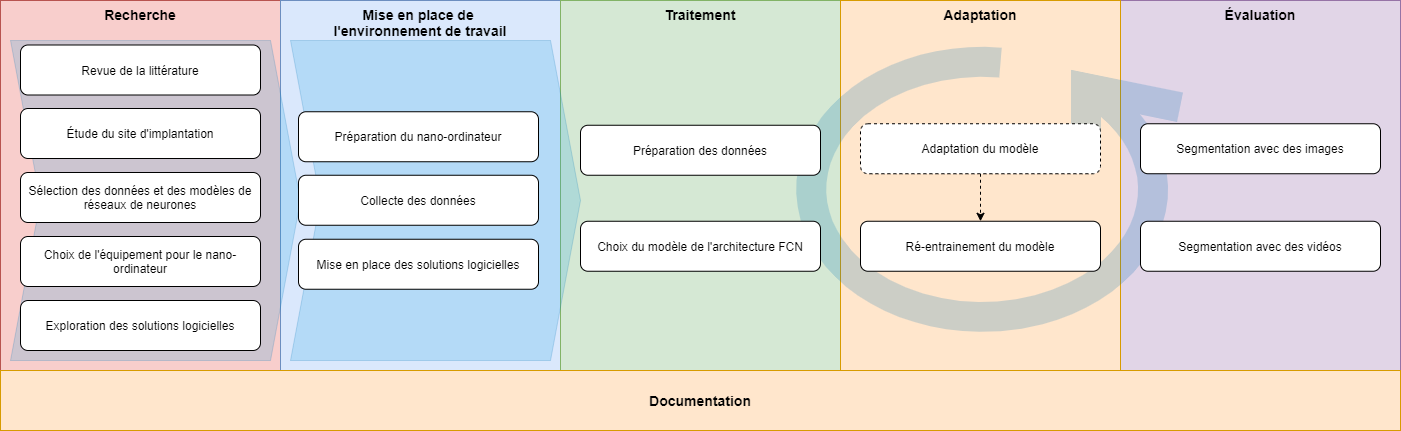
\includegraphics[width=0.75\textwidth]{methodologie_complexe}
    \caption{Organigramme de la méthodologie pour évaluer les performances après une phase d'adaptation théorique}
    \label{fig:methodologie_complexe}
\end{figure}
\par Mais sincèrement dans la pratique la méthodologie ressemblera plus à celle-ci: 
\label{methodologie_complexe_realiste}
\begin{figure}[H]
    \centering
    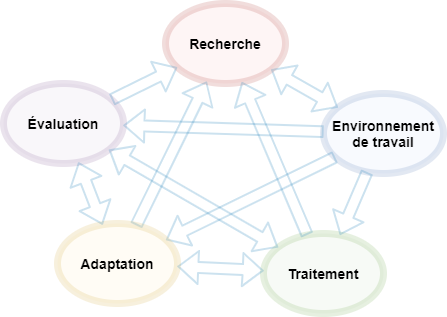
\includegraphics[width=0.65\textwidth]{methodologie_complexe_realiste}
    \caption{Organigramme de la méthodologie pour évaluer les performances après une phase d'adaptation réaliste}
    \label{fig:methodologie_complexe_realiste}
\end{figure}
\par Si chacun des blocs est explosé, chacun d'eux s'organise autour des activités suivantes: 
\label{methodologie_complexe_details}
\begin{figure}[H]
    \centering
    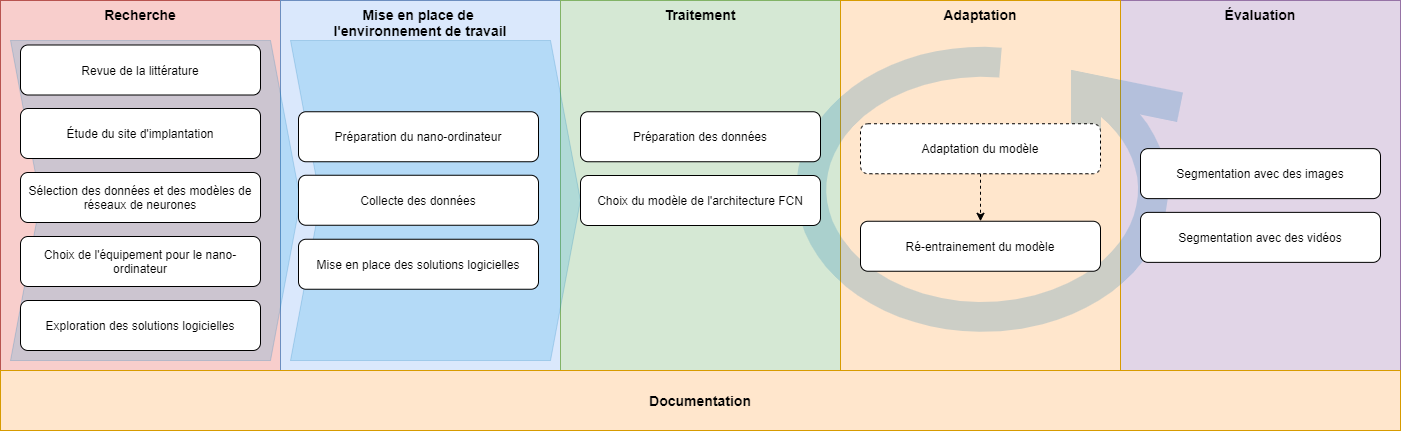
\includegraphics[width=1.0\textwidth]{methodologie_complexe_details}
    \caption{Organigramme des détails de la méthodologie pour évaluer les performances après une phase d'adaptation}
    \label{fig:methodologie_complexe_details}
\end{figure}
\par Voir l'organigramme de la figure \ref{fig:methodologie_complexe_details} pour la représentation graphique de la méthodologie, et dont les phases peuvent être résumées de la façon suivante:  
\begin{itemize}
   \item Recherche des références, des modèles et des données, ainsi que l'équipement pour le nano ordinateur et des logiciels nécessaires.
   \item Installation sur le Jetson nano du système d'exploitation, de l'environnement de développement et de tests pour l'inférence.
   \item Itération entre les étapes suivantes:
   \begin{itemize}
      \item Inférence avec le Jetson nano en utilisant les modèles et les sources de données sélectionnées.
      \item Adaptation des modèles à différentes résolutions d'images et à la zone d'étude.
      \item Traitement des données afin de les adapter au requis des modèles.
   \end{itemize}
\end{itemize}
\par Finalement, il est à noter  que le cheminement de l'essai a été entièrement documenté pendant tout le déroulement de l'essai.
\subsection{Documentation}
\par La méthodologie a été entièrement documenté pendant tout le déroulement de l'essai. Elle se retrouve pour référence dans un blog publique sur le site de "github.io" \footnote{https://vince7lf.github.io/}. Cette méthodologie de documentation permet entre autre, de très facilement documenter, de ne pas perdre des notes très importantes, de suivre le cheminement, de pouvoir retrouver des notes, mêmes si elles ont été effacées ou modifiées, puisque toute modification est sauvegardée dans un repository Git.
\par Par ailleur, tous les documents de rédaction LaTeX, les images, les scripts et code source qui ont été utiles et utilisés durant l'essai ont été géré dans un repository Git publique avec "github.com" \footnote{https://github.com/vince7lf/gae724}. 
\par Ces sources d'information viennent bonifier grandement ce rapport et il est même recommandé de s'y référer pour atteindre un certains niveau détails et de compréhension. 
\subsection{Recherche}

\subsubsection{Revue de littérature}
\noindent La recherche s'est concentrée sur des références traitantes des concepts du sujet de l'essai : la segmentation sémantique, le temps réel, et les nano ordinateurs. Le premier objectif a été de trouver si des études avaient déjà expérimenté le nano ordinateur, en particulier pour la segmentation de vidéos en temps réel. Pendant cette recherche, j'en ai profité pour effectuer une révision de l'évolution des réseaux de neurones convolutionnels entiers (\acrshort{fcn} \acrlong{fcn})  et des différentes architectures, et chercher d'autres solutions de détection de la route en temps réel grâce au \acrshort{fcn}. 
\vspace{\baselineskip}
\\
\noindent Il a été assez compliqué de trouver des références intégrant les nano ordinateurs. Comme l'objectif de l'essai est de valider les performances d'un nano ordinateur bien spécifique, les mots-clés "NVIDIA Jetson Nano" font partie de la stratégie de recherche. 
\vspace{\baselineskip}
\\
\noindent Les réseaux de neurones convolutifs entiers (\acrshort{fcn}) sont implicitement inclus dans les résultats puisque c'est le "state-of-art" actuellement pour répondre au besoin de la segmentation sémantique d'images.
\vspace{\baselineskip}
\\
\noindent Plus de 75 références ont été collectées. Une quarantaine ont été sélectionnées. Cette sélection peut se décomposer en trois catégories : les références se rapprochant le plus du sujet de l'essai; l'histoire et les antécédents des réseaux de neurones; du matériel éducatif pour étudier et manipuler les réseaux de neurones.
\vspace{\baselineskip}
\\
\noindent Je me suis intéressé aux références des années les plus récentes, autour de 2020, 2019 et 2018, car les avancées dans le domaine des réseaux de neurones sont très rapides. Par curiosité je suis allé aussi parfois voir dans les années bien plus éloignées, comme 1998, ou j'ai trouvé un article proposant une solution pour prédire la température de la surface de la route avec des réseaux de neurones.
\vspace{\baselineskip}
\\
\noindent Je n'ai pas pu trouver de références spécifiquement pour la déduction de l'état de la surface (mouillé, gelée, etc.) d'une piste multifonctionnelle (vélo, piéton). 
\vspace{\baselineskip}
\\
\noindent Il est intéressant de noter que la banque de données SCOPUS retourne plus de 11,000 documents avec l'expression "segmentation AND "real-time"". Il y en a plus de 700 uniquement pour l'année 2019. 
\subsubsection{Étude du site d'implantation}
\par Le nano ordinateur est destiné à être déployé sur le chemin de la piste multi-fonctionnelle du pont Jacques-Cartier. L'étude du site a permis de chercher à comprendre, parmis ses caractéristiques, les difficultés de son usage l'hiver. Il a été tenté de comprendre les défis et les raisons, techniques, politiques, sécuritaire, de pouvoir la conserver ouverte toute l'année. Une carte du site permet de montrer un exemple de configuration où et comment seront installés les nano-ordinateurs, et des images de ces  zones d'intérêt permet de "visualiser" ce qui sera interprété par le modèle. 
\par Un mot est réservé pour citer "L'Association des piétons et cyclistes du pont Jacques-Cartier" qui est un acteur actif pour le développement du transport actif dans cette région du Québec, et dont les membres sont des usagers habituels de la piste multifonctionnelle, même l'hiver.

\subsubsection{Sélection des données et des modèles de réseaux de neurones}
\noindent Les ressources mises à disposition par le constructeur du Jetson Nano, NVIDIA, ont été étudiées pour apprendre et tester le nano ordinateur. Parmi les plus intéressantes, on peut citer le "Jetson Nano Developer Kit", le "NVIDIA Deep Learning Institute", la communauté Jetson, les tutoriels, les "benchmarks". Des jeux de données sont fournis gratuitement.
\vspace{\baselineskip}
\\
\noindent En complément des ressources de NVIDIA, deux références scientifiques ont été principalement utilisées comme points de départ et base de travail pour l'essai, car leurs études ont été faites avec le Jetson Nano \parencite{nguyen_mavnet_2019} et \parencite{zheng_real-time_2020}. Beaucoup de références ont été publiées ces deux dernières années sur le sujet de la segmentation sémantique, ils existent donc de multiples alternatives inspirantes.
\vspace{\baselineskip}
\\
\noindent Il existe sur Internet des forums et des blogues dans lesquels des utilisateurs publient leurs expérimentations de la segmentation sémantique en temps réel avec le Jetson Nano \parencite{dustin_realtime_2019}, ou plus génériquement la segmentation sémantique. Des sites comme "modelzoo.co" et "kaggle.com" sont des entrepôts de modèles déjà entrainés. 
\vspace{\baselineskip}
\\
\noindent Une autre option est d'effectuer une recherche d'images ou de vidéos de la piste multifonctionnelle du pont Jacques-Cartier via les sites de recherche tels que Google. 
\vspace{\baselineskip}
\\
\noindent L'\acrlong{apcpontjc} existe depuis de nombreuses années pour promouvoir le transport actif et conserver la piste multifonctionnelle du pont Jacques Cartier ouverte durant l'hiver. Ils fournissent, via leurs sites Internet, des collections de vidéos et d'images qui pourront être utilisées. Il serait aussi possible d'entrer en contact avec l'association et leur demander de prendre de nouvelles vidéos au besoin. \parencite{association_des_pietons_et_cyclistes_du_pont_jacques-cartier_pontjacques-cartier365com_2020, association_des_pietons_et_cyclistes_pont_jacques-cartier_flickr_2020}
\vspace{\baselineskip}
\\
\noindent Les architectures des modèles \acrshort{fcn} sélectionnés pour l'essai sont résumés dans un tableau récapitulatif, incluant leur type, leur application et leurs jeux de données respectifs, précisant les différentes variantes entre résolutions et nombre d'images pas secondes (\acrshort{fps}).
\subsubsection{Choix de l'équipement pour le nano ordinateur}
\noindent L'objet d'étude de cet essai est un nano ordinateur. Un nano ordinateur est un ordinateur miniaturisé en taille, mais aussi limité en capacité. Il existe différents fabricants et modèles, de caractéristiques techniques variées, pour répondre à différents besoins. Le dernier né est le modèle "Jetson Nano" du fabricant "NVIDIA", disponible depuis juin 2019 au prix abordable de 99 \$US. La compagnie NVIDIA a conçu ce matériel spécialement pour différentes applications d'inférence de modèles d'apprentissage profond sur une plateforme mobile (drone) ou proche des données ("edge" en anglais). Ce modèle a été choisi afin de répondre à l'intérêt que suscitent ses capacités et ses limites. Une image du Jetson Nano et un tableau de ses caractéristiques techniques sont disponibles. 
\vspace{\baselineskip}
\\
\noindent L'architecture matérielle est étudiée et présentée avec l'aide d'images, de diagrammes et de textes explicatifs. Les éléments clés sont identifiés.
\vspace{\baselineskip}
\\
\noindent Afin d'optimiser les performances du nano ordinateur, une recherche des périphériques les plus adaptés pour répondre aux besoins de performance (et de budget) de l'essai est essentielle, telle que l'alimentation, le stockage, la caméra. Des images des périphériques sont incluses, et les caractéristiques principales sont présentées dans des tableaux.
\vspace{\baselineskip}
\\
\noindent Le matériel est commandé par le collaborateur de cet essai "Vision météo".
\subsubsection{Exploration des solutions logicielles}
\par De même que pour les périphériques, les solutions logicielles logiciels nécessires sont résumés dans un tableau, où il sera indiqué leur nom, leur version, les avantages et limitations, comme le système d'exploitation, l'environnement de développement, l'inférence, les logiciels de traitements vidéos et d'images. 

\subsection{Environnement de travail}

\subsubsection{Préparation du nano ordinateur}
\label{preparation_nano_ordinateur}
\par L'organigramme de la figure \ref{fig:preparation_nano_ordinateur} présente les activités qui composent la préparation du nano ordinateur. 
\begin{figure}[H]
    \centering
    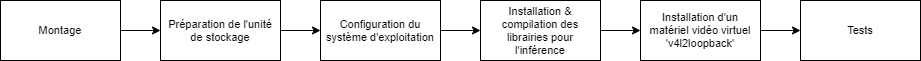
\includegraphics[width=1.0\textwidth]{preparation_nano_ordinateur}
    \caption{Préparation du nano ordinateur}
    \label{fig:preparation_nano_ordinateur}
\end{figure}
\myparagraph{Montage}
\par Le nano ordinateur est une carte mère livrée sans aucun périphérique ni même boitier. Vu que les performances logicielles dépendent des performances matérielles, surtout pour une unité telle qu'un nano ordinateur où les capacités matérielles sont très limitées, la première partie de l'essai a été allouée à la sélection des accessoires et périphériques qui vont permettre d'augmenter les performances, protéger et utiliser confortablement le nano ordinateur. 
\label{montage_nano_ordinateur}
\par L'organigramme de la figure \ref{fig:montage_nano_ordinateur} présente les activités qui composent le montage du nano ordinateur. 
\begin{figure}[H]
    \centering
    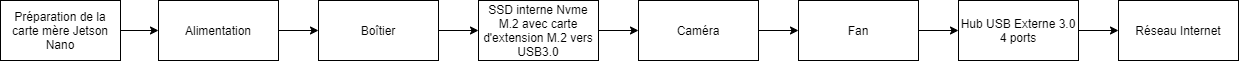
\includegraphics[width=1.0\textwidth]{montage_nano_ordinateur}
    \caption{Montage du nano ordinateur}
    \label{fig:montage_nano_ordinateur}
\end{figure}
\mysubparagraph{Préparation de la carte mère Jetson Nano}
\begin{figure}[H]
    \centering
    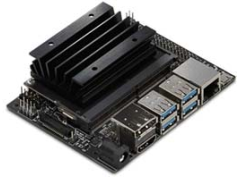
\includegraphics[width=0.5\textwidth]{jetson_nano}
    \caption{Carte mère du nano ordinateur}
    \label{fig:jetson_nano}
\end{figure}
\par Le nano ordinateur qui est livré dans sa boite est uniquement une carte mère, sans unité de stockage, ni boitier, clavier, souris, écran, capacité wifi, ou caméra. Il est uniquement livré avec un câble micro USB qui lui permet d'être démarré avec une alimitation minimale de 5 Volts/2Amp et ne consommer que 5 Watts. Aucun système d'exploitation n'est livré non plus. Vu que de l'objectif de l'essai est de tester les capacités du nano ordinateur et que la consommation sera de plus de 5Watt dues aux branchements de multiples périphériques, certaines "broches" sur la carte mère doivent être activées:  la broche J48 permet de brancher un adaptateur d'alimentation de 5Volts 4Amp au lieu de l'alimentation micro USB; et la broche J38 permet d'activer le PoE (Power-Over-Ethernet) afin d'hériter de l'alimentation du câble Ethernet. Aucune autre préparation sur la carte n'est nécessaire.
\mysubparagraph{Alimentation}
\begin{figure}[H]
    \centering
    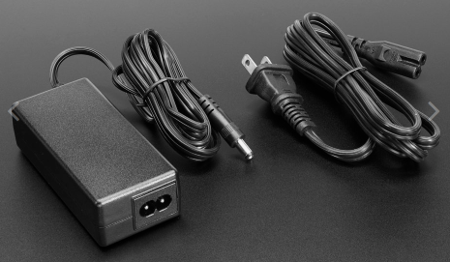
\includegraphics[width=0.5\textwidth]{alimentation}
    \caption{Adaptateur 5 volts 4 amps}
    \label{fig:alimenation}
\end{figure}
\par L'alimentation du nano ordinateur est l'élément matériel le plus important du système. De base le nano ordinateur est livré avec un câble micro USB, lui permettant d'être alimenté en 5Volt 2Amp. Mais le besoin en énergie augmente avec les périphériques qui s'accumulent, tel qu'une caméra. Il est prudent de choisir un adaptateur 5Volt 4Amp d'un fournisseur recommandé par NVIDIA, car un changement de puissance sensible en entrée impacte le fonctionnement opérationnel du nano ordinateur. Deux adaptateurs ont été utilisés, l'un recommandé, et l'autre non, afin de tester leur performance. 
\par Dans le cadre de l'essai, l'alimentation du nano ordinateur est utilisée pour alimenter la carte mère, qui comporte entre autres les CPUs, le GPU, le Hub USB 3.0 interne, le contrôleur Ethernet et le port HDMI. Mais aussi la caméra et  le ventilateur et optionnellement une carte d'extension M.2 NVMe. Afin d'assister l'adaptateur, un hub USB 3.0 externe a été utilisé pour brancher la souris, le clavier, et à un moment donné le dongle Wifi.
\mysubparagraph{Boitier}
\begin{figure}[H]
    \centering
    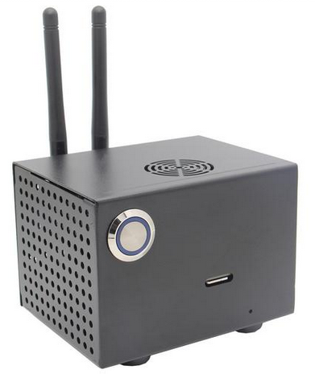
\includegraphics[width=0.45\textwidth]{boitier}
    \caption{Boitier pour le nano ordinateur}
    \label{fig:boitier}
\end{figure}
\begin{figure}[H]
    \centering
    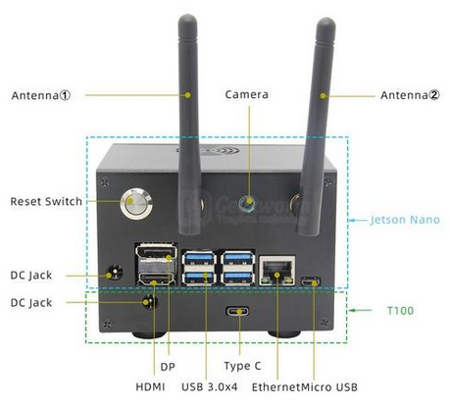
\includegraphics[width=0.5\textwidth]{boitier_back}
    \caption{Vue arrière du boitier pour le nano ordinateur}
    \label{fig:boitier_arriere}
\end{figure}
\par Afin de protéger le nano ordinateur durant l'essai et l'utiliser dans les conditions les plus proches de son futur mode d'opération, il a été installé dans un boitier en métal. Le boitier a été choisi en tenant compte qu'une carte d'extension pour un SSD interne sera installée, ainsi qu'une caméra et un ventilateur. Durant l'essai le nano ordinateur sera manipulé très fréquemment en raison d'un manque d'espace réservé dans la maison. Le boitier permet donc d'éviter de manipuler le matériel et les connecteurs, les protège, évitant de risquer de les briser, et donc ajouter des délais à l'essai. 
\mysubparagraph{Unité de stockage}
\par Le nano ordinateur est conçu pour fonctionner avec un système d'exploitation hébergé sur une carte microSD. Il existe différentes cartes microSD, et certaines sont  beaucoup plus performantes que les autres. Malheureusement les cartes microSD ne sont pas destinées à exécuter un système d'exploitation à temps plein, et leur espérance de vie reste très limitée.  Étant donné que l'objectif du nano ordinateur est d'être en service continuelle à l'extérieure, l'utilisation un disque SSD interne comme alternative semble logique.
\par\underline{Carte microSD}
\par Il existe différentes cartes microSD, de multiples constructeurs, et pour différents usages, mais généralement destiné pour stocker des images et vidéos directement par les appareils multimédias. Leur conception est faite pour la manipulation de gros blocs de données, et non des petits fichiers. Trois cartes microSD 
seront évaluées:
{
    \renewcommand*{\arraystretch}{1.4}
    \begin{table}[ht]
    \centering
    \caption{Cartes microSD}\label{table:cartes_microSD}
    \vspace{0.3em} % Adjust the height of the space between caption and tabular
    \begin{tabular}{l}
        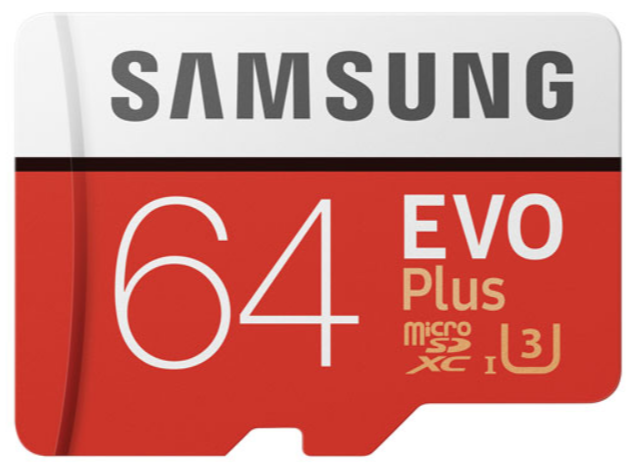
\includegraphics[width=0.15\textwidth]{micro_sd_evo_plus} microSD Samsung EVO 64Gb Plus XC I Grade 3 Class 10\\
        
\includegraphics[width=0.15\textwidth]{micro_sd_evo} microSD Samsung EVO 64Gb Select XC I Grade 3 Class 10\\
        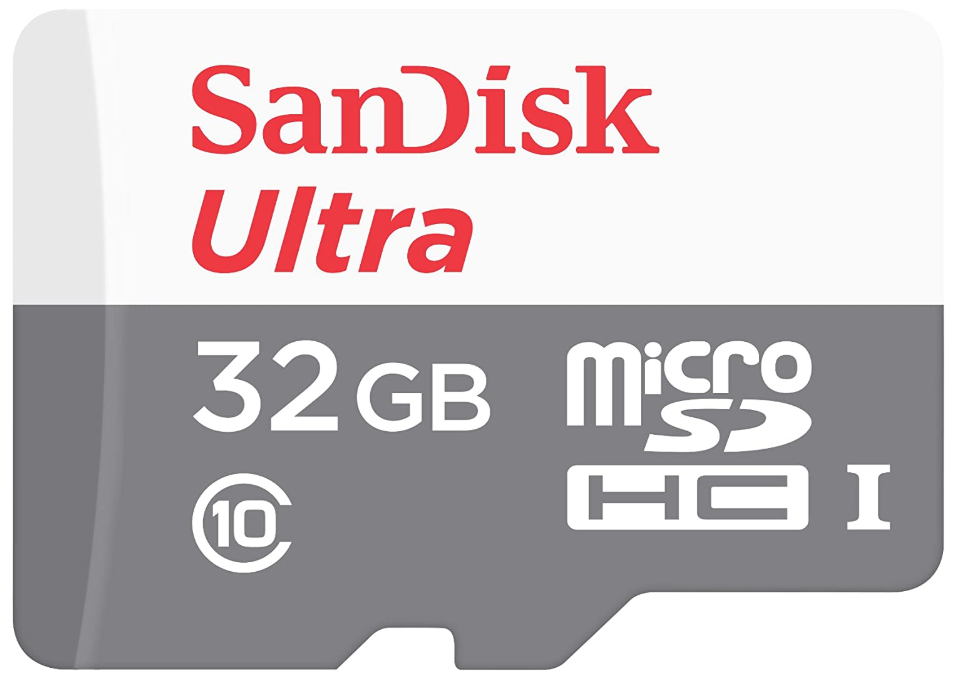
\includegraphics[width=0.15\textwidth]{Microsd card Scan Disk Ultra 32Gb class 10 HC I} microSD Scan Disk Ultra 32Gb HC I Class 10\\
    \end{tabular}
    \end{table}
}
{\color{red}\todo{fix le tableau}}
\par\underline{Disque SSD}
% \mysubparagraph{SSD interne Nvme M.2 avec carte d'extension M.2 vers USB3.0}
% \par Pour un appareil destiné à être continuellement en service et à l'extérieure, l'unité de stockage doit être non seulement performante, mais aussi endurante. Un disque SSD interne pour un nano ordinateur est soit une carte d'extension M.2 NVMe ou SATA (selon la carte d'extension), connecté au port PCIe ou USB. Les SSD internes Samsung 970 EVO 250GB NVMe M.2 et Samsung 860 EVO M.2 500GB SATA seront évalués. À noter qu'une carte microSD est tout de même nécessaire pour "bootstrapper" le système d'exploitation. Il n'est pas nécessaire d'avoir une carte microSD performante puisqu'elle n'est utilisée que pour démarrer le système qui se trouve sur le SSD interne. 
\par Un disque SSD et une carte microSD sont différents type de matériel pour différents usages. Le disque SSD est plus adapté pour manipuler les petits fichiers et héberger un système d'exploitation. Il est aussi plus résilient à long terme. C'est donc une option qui ne doit pas être négligée dans le contexte de tests de performance, encore plus avec un nano ordinateur dont les capacités matérielles sont limitées, et qui est un appareil destiné à être continuellement en service et à l'extérieure. L'unité de stockage doit être non seulement performante, mais aussi endurante. Néanmoins, il y a un contreparti important dans la situation d'un nano ordinateur: la consommation d'énergie. Un SSD interne va demander plus d'énergie qu'une carte microSD, et si le nano ordinateur n'est pas capable de gérer correctement les besoins en énergie de ses extensions matériels, le SSD interne risque d'échouer en pleine opération et le nano ordinateur devenir non fonctionnel soudainement.
\par Un disque SSD interne pour un nano ordinateur est soit une carte d'extension M.2 NVMe ou SATA (selon la carte d'extension), connecté au port PCIe ou USB. Les SSD internes Samsung 970 EVO 250GB NVMe M.2 et Samsung 860 EVO M.2 500GB SATA seront évalués.
\begin{figure}[H]
    \centering
    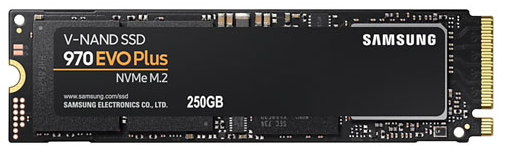
\includegraphics[width=0.5\textwidth]{Samsung 970 EVO Plus 250GB M.2 NVMe Internal Solid State Drive}
    \caption{Disque SSD NVMe M.2 interne 250GB}
    \label{fig:disquessd}
\end{figure}
\par Il y a deux choix qui ont été retenus pendant l'essai pour brancher un SSD interne au nano ordinateur: soit via une carte d'extension M.2 MVMe, et connecté via le Hub USB, soir via une carte d'extension M.2 NVMe connectée au port PCIe interne du nano ordinateur, normalement destinée à une carte d'extension Wifi.
\par Concernant le disque SSD M.2 NVMe connecté à la carte d'extension M.2 via le Hub USB 3.0 interne, le système L4T de NVIDIA ne supporte pas les SSD M.2 NVMe connecté au port USB \footnote{À noter que la carte d'extension T100 est discontinuée et remplacée par la T130}. Il n'est pas reconnu / détecté, il est donc impossible de le formater, de le partitionner, de l'utiliser. Comme il serait risqué pour l'essai de se lancer dans la recompilation du kernel du L4T, une alternative trouvée sur le développeur forum de NVIDIA est de passer par un adaptateur M.2 MVMe connecté au port PCIe interne.
\par Malheureusement cette alternative a rapidement été abandonnée. Il a été possible de démarrer et installer le système d'opération sur le SSD M.2, et faire quelques tests, mais pour une raison inconnue, le système n'était pas stable et devenait non opérationnel assez rapidement, le système perdant la connexion au SSD. La durée la plus longue de stabilité observée a été de moins 30 minutes. Une hypothèse est une baisse d'énergie qui survient à un moment et qui impacte l'alimentation du SSD, chaque volt et milliampère étant important pour la stabilité du nano ordinateur. De plus, le raccordement du câble de la carte d'extension M.2 NVMe PCIe avec le SSD M.2 NVMe est très compliqué et risqué pour le câble lui-même. Une autre limitation importante est que cette solution ne permet pas d'utiliser le boitier, car le SSD M.2 ne rentre pas et ne peut même pas être fixé. 
\par Différentes options pour optimiser l'alimentation ont été explorées: utiliser un HUB USB externe et auto alimenté; brancher un câble Ethernet au lieu d'utiliser un Dongle Wifi; allumer le ventilateur dès le démarrage du nano ordinateur; et l'option de fournir 6Amp directement supportée par la carte mère via les pins; explorer les solutions sur les forums de discussion \footnote{\url{https://www.kingston.com/en/community/articledetail/articleid/48543}} \footnote{\url{https://geekworm.com/products/nvidia-jetson-nano-nvme-m-2-ssd-shield-t100-v1-1}}.
\mysubparagraph{Caméra}
\begin{figure}[H]
    \centering
    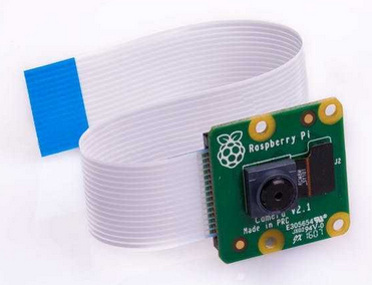
\includegraphics[width=0.40\textwidth]{camera}
    \caption{Caméra}
    \label{fig:camera}
\end{figure}
\par L'objectif du nano ordinateur est d'être utilisé pour détecter continuellement les délimitations de la piste cyclable. Il est évident qu'une caméra doit donc faire partie du système et faire partie de l'évaluation des performances. Néanmoins, durant le déroulement de l'essai, la caméra sera très peu utilisée. En effet il n'est pas évident d'être dans un mode de développement directement sur le terrain. Un matériel vidéo virtuel sera utilisé pour simuler la caméra et alimenter l'inférence avec des vidéos préenregistrées, permettant ainsi d'évaluer les performances de l'inférence avec des vidéos, même si d'un point de vue performance matérielle l'utilisation ne sera pas équivalente. Les performances matérielles de l'inférence en temps réel seront évaluées avec la caméra, même si la vue de la caméra n'est pas la piste cyclable, ce qui n'est pas important pour ce test, peu importe ce qui est détecté. 
\par la caméra qui a été sélectionnée est la version 2 de celle du fournisseur Raspberry Pi, le concurrent directe du nano ordinateur NVIDIA Jetson Nano. Cette caméra a été épprouvée avec le temps, est performante, elle semble être la plus adaptée pour ce genre de projet. 
\mysubparagraph{Ventilateur}
\begin{figure}[H]
    \centering
    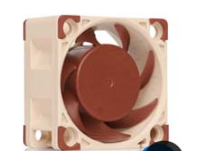
\includegraphics[width=0.35\textwidth]{fan}
    \caption{Ventilateur}
    \label{fig:fan}
\end{figure}
\par Un système informatique a besoin d'un ventilateur pour évacuer la chaleur produite par ses processeurs et les autres éléments électroniques, et éviter une faute opérationnelle et des bris de matériel. L'objectif du nano ordinateur étant d'être opérationnel continuellement, et ses éléments étant contenus dans un boitier, il est encore plus indispensable d'installer un ventilateur. Le ventilateur choisi a pu être installé dans le boitier, même si le boitier ne possède de support pour le fixer. Le ventilateur est capable de démarrer automatiquement au besoin, mais il est volontairement démarré manuellement dès que le nano ordinateur est démarré. Cela évite que la chaleur ne s'accumule, qu'elle soit tout de suite ventilée à l'extérieure, évitant un risque de surchauffe, la capacité du ventilateur étant tout de même limité (petit modèle).
\mysubparagraph{Hub USB externe 3.0 4 ports}
\begin{figure}[H]
    \centering
    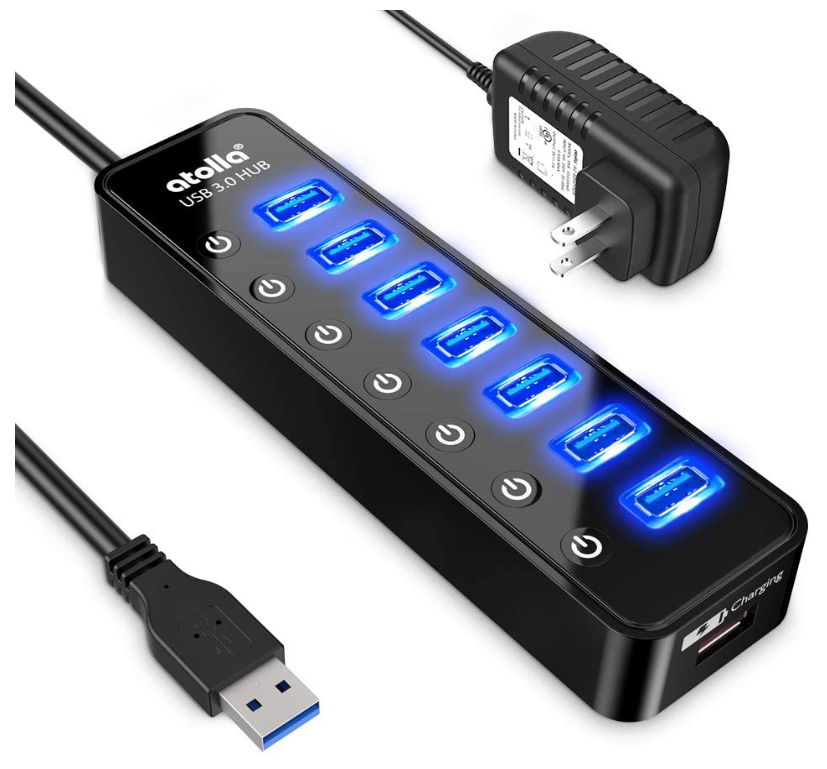
\includegraphics[width=0.4\textwidth]{Powered USB Hub 3.0, Atolla 7-Port USB Data Hub Splitter with One Smart Charging}
    \caption{Hub USB 3.0 externe autoalimenté}
    \label{fig:hubusb}
\end{figure}
\par Le nano ordinateur comprend un hub USB 3.0 4 ports internes, les 4 ports étant connectées via le même contrôleur. Ce hub consomme de l'énergie pour alimenter les périphériques qui y sont connectés, comme un SSD interne ou un dongle Wifi, et gérer l’ échange de données. Afin de minimiser les besoins en alimentation et optimiser le plus possible le transfert de données, la souris, le clavier et le dongle USB ont été branchés a un hub USB 3.0 externe autoalimenté. Malheureusement cette option complexifie le déploiement sur le terrain du nano ordinateur. L'alternative pour s'en passer est d'utiliser un câble Ethernet, PoE préférablement, à la place d'un dongle Wifi qui est très gourmant en termes de besoin en alimentation, et chauffe rapidement.
\mysubparagraph{Réseau Internet}
\par Le nano ordinateur comprend un contrôleur Ethernet pour brancher un câble réseau et se brancher sur Internet. Selon la configuration de la carte mère, le nano ordinateur peut hériter de l'alimentation via Ethernet (PoE), via la broche J38. Il comprend aussi un port PCIe interne qui permet de brancher une carte d'extension Wifi. L'autre alternative étant de passer par un dongle USB Wifi, ou un périphérique Wifi externe connecté au port USB. 
\par Dans le cadre de cet essai, le périphérique Wifi externe USB a été utilisé en premier puisque déjà disponible. Malheureusement les performances étaient assez décevantes, le réseau Wifi à la maison n'étant pas non plus très performant dans la pièce ou le nano ordinateur était installé (table de la cuisine). Un débit d'environs 5Mbits était disponible. Par curiosité un dongle USB Wifi a été acquis, mais autant décevant. La meilleure alternative pour améliorer le déroulement de l'essai a été de tirer un câble Ethernet et d'installer un router secondaire, et de brancher le nano ordinateur a ce nouveau router. L'accès Internet a été plus stable et de bien meilleure qualité, la connexion étant d'environs 11Mbs. 
\par Le PoE n'a pas été évalué. 
\myparagraph{Préparation de l'unité de stockage}
Le nano ordinateur est conçu pour fonctionner avec une microSD, et NVIDIA fournit uniquement de la documentation à cet effet. L'option d'utiliser un disque SSD interne est disponible sur Internet, mais n'est pas supporté officiellement par NVIDIA. Il existe néanmoins des articles à ce sujet dans le forum des développeurs\footnote{\url{https://forums.developer.nvidia.com/t/how-to-connect-ssd-to-jetson-nano/74053}}. 
\mysubparagraph{Carte microSD}
\par NVIDIA fournit de la documentation très claire et simple afin de préparer la carte microSD (formattage) et installer l'image du JetPack.\footnote{\url{https://developer.nvidia.com/embedded/learn/get-started-jetson-nano-devkit#write}}.
\mysubparagraph{Disque SSD}
\par La procédure d'installation pour installer JetPack sur le SSD interne est disponible sur le site "jetsonhacks.com"\footnote{\url{https://www.jetsonhacks.com/2019/09/17/jetson-nano-run-from-usb-drive/}}. À noter qu'une carte microSD est tout de même nécessaire pour "bootstrapper" le système d'exploitation. Il n'est pas nécessaire d'avoir une carte microSD performante puisqu'elle n'est utilisée que pour démarrer le système qui se trouve sur le SSD interne. 
\myparagraph{Configuration du système d'exploitation}
\par La première fois que le système démarre, le système Ubuntu Linux For Tegra (L4T) doit être configuré avec toutes les options personnalisées (langue, clavier, timezone, etc.).
\myparagraph{Installation \& compilation des librairies pour l'inférence}
\par Les librairies pour la segmentation sémantique 
d'images et de vidéos via l'inférence de modèles déjà préparée sont mises à disposition par NVIDIA via un projet dans GitHub. La documentation pour l'installation et l'inférence est disponible directement dans la page GitHub. 
\myparagraph{Installation d'un matériel vidéo virtuel 'v4l2loopback'}
\par L'inférence fournie par NVIDIA est conçue pour utiliser la caméra du nano ordinateur. Ce qui n'est pas forcément "pratique" pour évaluer la segmentation sémantique d'une vidéo d'une piste cyclable. Heureusement un matériel vidéo virtuel permet de simuler la caméra et d'alimenter l'inférence avec une vidéo enregistrée, au lieu de la caméra. La contrepartie concerne l'évaluation des performances:  en effet la caméra demande plus de puissance au nano ordinateur que le simulateur logiciel.
\myparagraph{Tests}
\par Afin de s'assurer que le nano ordinateur est prêt pour être évalué, des tests matériels et logiciels sont  effectués une fois le système monté et stabilisé. Les résultats des tests servent de référence pour évaluer l'état de santé du nano ordinateur. 
\subsubsection{Collecte des données}
\par 
\vspace{1\baselineskip}
\par 
\subsubsection{Mise en place des solutions logicielles}
\myparagraph{Jetson Nano}
\vspace{0.5\baselineskip}
\\
\noindent Le nano-ordinateur est destiné à l'inférence. NVIDIA fournit tout un système d'installation, qui est nommé JetPack, et qui contient un système d'exploitation basée sur Ubuntu, "\acrlong{l4t}" \acrshort{l4t}), la plateforme applicative et les librairies nécessaires pour l'inférence, tels que Python, pytorch, les modèles préentrainés au format \acrshort{onnx}, le compilateur CUDA, et le \acrshort{sdk} TensorRT.
\myparagraph{Calcul Québec}
\vspace{0.5\baselineskip}
\\
\noindent Le nano-ordinateur est destiné à l'inférence, et non l'entrainement d'architectures. Il n'est pas non plus destiné à être un environnement de développement. Un autre environnement de travail est donc nécessaire pour développer, et doit posséder les capacités matérielles (\acrshort{gpu}s, mémoires, espace de stockage) et logicielles (librairies) pour entrainer une architecture. Le professeur Mickaël Germain, directeur de projet, m'a présenté l'environnement de Calcul Québec. Celui-çi fournit un espace de travail scientifiques destiné aux chercheurs et aux universitaires, qui m'a permit  de pouvoir travailler avec l'apprentissage profond, compiler un fork de torchvision, réentrainer des architetures, générer les versions \acrshort{onnx}, et ainsi contourner les limitations du nano-ordinateur. Avoir accès à cet environnement de travail a été un élément clé dans le cadre de cet essai.
\mysubparagraph{Compte Calcul Québec}
\vspace{0.5\baselineskip}
\\
\noindent Calcul Québec mets à disposition des ressources matérielles puissantes et l'accès a des libraires de haute technologie telle que pour l'apprentissage profond, permettant d'avoir un environnement de travail professionnel et performant rapidement. Les ressources matérielles à disposition sont des grappes de serveurs, de \acrshort{cpu}s et \acrshort{gpu}s de différents types, ainsi que de l'espace de stockage. Les librairies sont disponibles via un repository privé, et lorsque certaines étaient manquantes (\acrshort{onnx} et onnxruntime), j'ai fait une demande par courriel. L'administrateur a pu rendre disponible l'une des deux (\acrshort{onnx}), la seconde (onnxruntime) étant beaucoup plus complexe a installé, pour l'avoir tenté sur le nano-ordinateur. 
\vspace{0.5\baselineskip}
\\
\noindent L'autre avantage de l'environnement de Calcul Québec est la mise à disposition de Jupyter Notebook, afin de tester rapidement du code Python. Par contre il n'est pas conseillé d'exécuter du code nécessitant des délais, tels que l'entrainement d'une architecture. 
\vspace{0.5\baselineskip}
\\
\noindent L'un des irritants est de ne pas pouvoir exécuter un conteneur Docker tel quel. Il faut le convertir au format Singularity. Dans le cadre du projet cela m'aurait facilité la tâche, car NVIDIA fournit des conteneurs Docker prêts à l'utilisation pour le réentrainement. Je n'ai malheureusement pas pris le temps et la chance de convertir un conteneur Docker au format Singularity. Je ne sains pas si c'est une activité assez simple ou complexe, mais du peu que j'ai lu cela semble assez "rapide".
\mysubparagraph{Jupyter Notebook}
\vspace{0.5\baselineskip}
\\
\noindent Le besoin de tester du code Python est toujours nécessaire. La console Python n'étant vraiment pas conviviale, un environnement Jupyter Notebook est un compromis incontournable. Heureusement Calcul Québec fournit un accès à des notebooks depuis Internet, permettant en plus d'hériter de leur environnement de travail. Il est à noter que les notebooks n'ont pas été utilisés pour entrainer une architecture ou générer les versions \acrshort{onnx}, mais de tester du code Python simple, comme visualiser des images, transformer des tensors, et évaluer la segmentation prédite générée avec le vérité terrain (\acrshort{gt}). 
\paragraph{NVIDIA}
\mysubparagraph{Compte NVIDIA}
\vspace{0.5\baselineskip}
\\
\noindent NVIDIA mets à disposition tout un écosystème éducatif permettant aux développeurs et aux chercheurs d'obtenir de l'aide au sujet de leur produit et librairies. Dans le cadre de l'essai, un compte NVIDIA a été créé, permettant d'accéder au forum de développeurs, et les conterneurs Docker par exemple. Il est aussi possible d'accéder à du matériel éducatif grâce à l'institut DeepLearning de NVIDIA, dont l'accès a été commandité par le professeur Mickaël Germain, directeur de projet. Le forum de développeurs a été un outil utile dans le cadre de ce projet, car le dépôt d'une question m'a permis de me débloquer. Je n'étais pas capable de regénérer la version \acrshort{onnx} à partir du code source et de la documentation fournie par NVIDIA pour une architecture \acrshort{fcn}. Le développeur principal de l'application a répondu et m'a guidé dans la résolution du problème. Les autres ressources ont eu un impact limité dans le cadre de ce projet, puisque par exemple le conteneur Docker et DIGITS n'ont pas pu être utilisé. Le code source des architectures est disponible sans nécessiter de compte, de même que les \acrshort{sdk}s Jetpack.
\mysubparagraph{NVIDIA DIGITS}
\vspace{0.5\baselineskip}
\\
\noindent NVIDIA fournit aux développeurs un environnement visuel permettant de réentrainer les architectures \acrshort{fcn} qu'ils fournissent avec leurs propres dataset. Cet environnement se nomme DIGITS. Malheureusement il est nécessaire d'avoir son propre matériel, le système d'exploitation Ubuntu 18.04 LTS, d'avoir au moins un \acrshort{gpu}. DIGITS ne s'installe pas sur le nano-ordinateur, ni sous Windows, ni avec la version "\acrshort{wsl}" (\acrlong{wsl}). Cette option a donc été abandonnée rapidement. 
\mysubparagraph{Conteneur Docker NVIDIA}
\vspace{0.5\baselineskip}
\\
\noindent NVIDIA fournit aux développeurs des conteneurs Docker, avec tout ce qui est nécessaire pour réentrainer une architecture et regénérer une version \acrshort{onnx}, par exemple. Malheureusement la capacité du nano-ordinateur ne permet pas de travailler efficacement avec un conteneur Docker, le nano-ordinateur devient sans réponse, nécessitant un redémarrage forcé. Cette option a donc été aussi abandonnée rapidement. 
\mysubparagraph{NVIDIA DeepStream}
\vspace{0.5\baselineskip}
\\
\noindent Durant le déroulement de l'essai, NVIDIA a mis à disposition un environnement d'apprentissage profond, nommé "DeepStream", facilitant la conception et la génération de modèles, jusqu'à l'inférence. Cet outil n'a pas été évalué, mais pourrait être un outil alternatif pour réentrainer une architecture.
\subsection{Évaluation}
\label{metho_eval}
\begin{figure}[H]
    \centering
    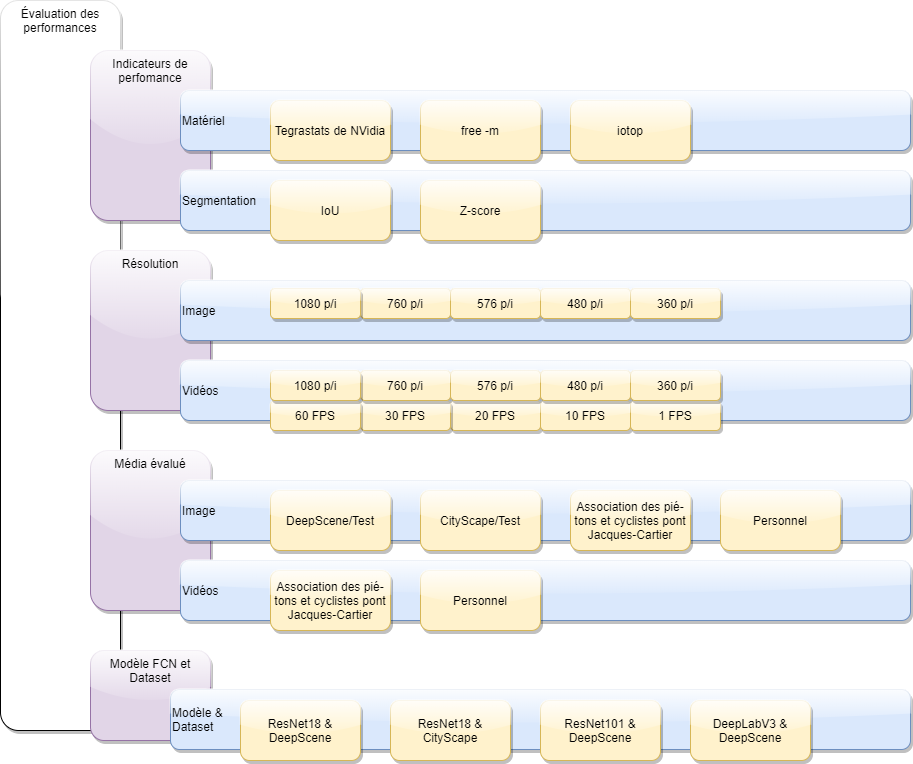
\includegraphics[width=1.0\textwidth]{metho_eval_perf_round_glass_shadow}
    \caption{Éléments pour l'évaluation des performances}
    \label{fig:metho_eval}
\end{figure}
\subsubsection{Stratégie de test}
\par L'objectif principal de l'essai est de déterminer la capacité et les limites du nano ordinateur d'inférer en temps réel des modèles de réseau de neurones à convolution entier pour la segmentation sémantique de vidéos. La stratégie qui sera appliquée sera de tester avec divers modèles et divers niveaux de qualité vidéos, en espérant trouver le compromis qui répond le mieux à cet objectif.
\begin{enumerate}
   \item \label{metho:testbaseinférence} Afin de s'assurer du bon fonctionnement du nano ordinateur et d'avoir des résultats de référence propre à notre environnement, l'inférence sera testée avec des modèles existants et pré entrainés pour la segmentation sémantique, avec les images et les vidéos provenant des références, et dont les caractéristiques et les résultats sont disponibles. 
   \item \label{metho:testbaseinférencesite} En espérant que les tests de l'étape \#\ref{metho:testbaseinférence} précédente donnent les résultats documentés dans les articles de références, ils seront repris avec les mêmes modèles, mais avec les images et les vidéos du site d'étude possédant la meilleure qualité acquise (1080p/i, 30FPS). Les données sources (images et vidéos) devront subir certains prétraitements à ce effet, afin de répondre aux requis des modèles.
   \item \label{metho:testdevinférencesite} Selon les résultats de l'étape \#\ref{metho:testbaseinférencesite}, les tests se concentreront sur l'inférence avec des vidéos, en réduisant progressivement la résolution (760p/i, 576p/i, 480p/i, 360p/i) et le nombre d'images par seconde (20FPS, 10FSP, 1FPS).
   \item Les étapes intermédiaires de l'étape \#\ref{metho:testdevinférencesite} précédente seront de 1) valider les résultats de l'inférence avec des images avant de tester avec les vidéos, et 2) évaluer si les modèles de réseaux de neurones à convolution entiers doivent et/ou peuvent être adaptés facilement, en tenant compte de l'échéancier de l'essai, et ce afin de répondre à l'objectif principal.
\end{enumerate}
\subsubsection{Stratégie de collecte des indicateurs de performance}
\par La méthodologie de la collecte des indicateurs est la suivante\footnote{\url{https://vince7lf.github.io/2020/05/26/metrics.html}}: 
\begin{itemize}    
    \item La collecte est démarrée après un démarrage frais, manuellement, via un script shell, qui exécute chaque outil, et attend l'interruption du test. 
    \item Chaque outil qui est utilisé pour collecter les mesures, possède son propre fichier.
    \item La date et l'heure de chaque indicateur collecté sont précisées.
    \item Afin de faciliter la documentation et l'analyse du test, des points d'intérêt sont ajoutés dans un fichier séparé pour marquer un moment particulier du test, avec la date, l'heure et un libellé. Ce point d'intérêt est fait grâce à une commande "shell" qui vient ajouter une trace dans ce fichier.
    \item Chaque indicateur est collecté toutes les secondes.  
    \item Une fois le test complété, la collecte est arrêté manuellement. 
    \item Chaque fichier est ensuite transformé en fichier CSV, via des commandes shell.
    \item À partir des fichiers CSV un script Python génère les graphiques automatiquement. 
\end{itemize}
\par Chaque indicateur est une colonne du fichier CSV. Il existe le même nombre d'indicateurs à tout moment. La date et l'heure sont un champ. 
\par Avant tout début de tests, la collecte est démarrée sans activité autre que la collecte des indicateurs. Cela permet de prendre une base de référence sans aucune charge.
\par Ensuite les tests débutent. 
\par Les indicateurs collectés permettent de créer des graphiques qui montrent la progression de chacun.
\par Les performances matérielles du Jetson Nano sont évaluées grâce à différentes commandes : "tegrastats" fournis par NVIDIA, "free -m" et "iotop".
\par Les performances de la segmentation sont évaluées grâce au IoU et au z-score pour la classe du chemin / route. Une fonction Python est utilisée. Les fonctions IoU et le z-score utilisent l'image prédite (généré par le modèle FCN) et l'image vérité terrain ("ground truth"). Les images originales sont donc présélectionnées selon leur intérêt et l'image vérité terrain ("ground truth") créée. L'image prédite et vérité terrain ("ground truth") doivent utiliser la même palette de couleurs et doivent être de la même résolution. Pour les images qui ne possèdent pas d'image vérité terrain ("ground truth"), cell-ci est créée à la main avec l'éditeur "Gimp". Comme la résolution de la segmentation de l'image prédite par le modèle de NVIDIA est très faible ("carrée"), l'image vérité terrain ("ground truth") ne sera pas précise au pixel prêt. Le besoin est d'évaluer et non d'entrainer, l'importance de la précision de la classification est moindre dans ce cas. 
\subsubsection{Segmentation avec des images}
\myparagraph{Préparation et post-traitement}
\vspace{\baselineskip}
\\
\noindent Afin de pouvoir mesurer les performances de la segmentation (IoU, F1 score), les classes et la palette de couleur entre l'image vérité terrain (\acrshort{gt}) et celles prédites doivent être les mêmes.
\vspace{\baselineskip}
\\
\noindent L'image vérité terrain (\acrshort{gt}) du jeu de donnée original DeepScene ne possède pas la même palette de couleur ni exactement les mêmes classes que celle de l'architecture.
\vspace{\baselineskip}
\\
\noindent Un travail d'uniformisation est nécessaire avant la segmentation, qui est résumée dans le tableau \ref{table:classes_palette_couleur}.
{
    \renewcommand*{\arraystretch}{1.4}
    \begin{table}[h]
    \centering
    \caption{Classes et palettes de couleur}\label{table:classes_palette_couleur}
    \vspace{0.1em} % Adjust the height of the space between caption and tabular
    \begin{tabular}{{@{}|p{4em}|p{6em}||p{4em}|p{6em}||p{4em}|p{6em}|@{}}}
        \hline
        \multicolumn{2}{|c||}{\textbf{DeepScene}} & \multicolumn{2}{c||}{\textbf{NVIDIA}} & \multicolumn{2}{c|}{\textbf{Consolidée}} \\
        \hline
        \multicolumn{1}{|l|}{\textbf{Classes}} & \multicolumn{1}{c||}{\textbf{RGB}} & \multicolumn{1}{l|}{\textbf{Classes}} & \multicolumn{1}{c||}{\textbf{RGB}} & \multicolumn{1}{l|}{\textbf{Classes}} & \multicolumn{1}{c|}{\textbf{RGB}} \\
        % \thead{Classes \\ DeepScene} & \thead{RGB \\ DeepScene} & \thead{Classes \\ NVIDIA} & \thead{RGB \\ NVIDIA} & \thead{Classes \\ consolidées} & \thead{RGB \\ consolidées} \\
        \hline
        \hline
        Road & 170-170-170 & Trail & 200-155-75 & Trail & \textcolor{red}{170-170-170}\\
        \hline
        Grass & 0-255-0 & Grass & 85-210-100 & Grass & \textcolor{red}{0-255-0}\\
        \hline
        Vegetation & 102-102-51 & Vegetation & 15-100-20 & Vegetation & \textcolor{red}{102-102-51}\\
        \hline
        Tree & 0-60-0 & - & - & \textcolor{red}{Vegetation} & \textcolor{red}{102-102-51}\\
        \hline
        Sky & 0-120-255 & Sky & 0-120-255 & Sky & 0-120-255\\
        \hline
        Obstacle & 0-0-0 & Obstacle & 255-185-0 & Obstacle & \textcolor{red}{0-0-0}\\
        \hline
    \end{tabular}
    \end{table}
\vspace{\baselineskip}
\\
\noindent De plus, l'image segmentée prédite par l'architecture ne possède pas précisément la même palette de couleur que celle qui est configurée, il y a quelques différences minimes dans les codes couleurs RGB (par exemple 0-119-255 au lieu de 0-120-255), mais qui doivent être arrangée afin de pouvoir être correctement évaluées. 
\vspace{\baselineskip}
\\
\noindent Un travail de traitement de l'image segmentée prédite est nécessaire avant l'évaluation de la segmentation.
\myparagraph{Segmentation et évaluation}
\vspace{\baselineskip}
\\
\noindent Afin de tester la performance de la segmentation du modèle, deux images du jeu de données de DeepScene sont utilisées, car ce jeu contient déjà les images vérités terrain (\acrshort{gt}), un gain de temps non négligeable dans le cadre de l'essai. Uniquemement la classe "Trail" est évaluée.
\vspace{\baselineskip}
\\
\noindent L'architecture fournit à l'utilitaire "segnet-console" est "fcn-resnet18-deepscene-576x320" \footnote{\url{segnet-console -{}-network=fcn-resnet18-deepscene -{}-visualize=mask -{}-alpha=10000 images/city_0.jpg output.jp}}. 
\vspace{\baselineskip}
\\
\noindent Un script Python\footnote{\url{https://gist.github.com/ilmonteux/8340df952722f3a1030a7d937e701b5a}} est utilisé afin de mesurer le \acrshort{iou} et le F1 score de la classe de l'image prédite par l'architecture.
\subsubsection{Segmentation avec des vidéos}
\myparagraph{Préparation et pré-traitement}
\par L'évaluation de la segmentation avec des vidéos va s'effectuer non pas avec la caméra, mais avec un matériel vidéo virtuel. En effet, il n'est pas réaliste de pouvoir travailler sur le terrain. La commande "segnet-camera" permet de fournir en option le matériel qui doit être utilisé, par exemple "/dev/video0" pour la caméra. Le module "v4l2loopback"\footnote{\url{https://github.com/umlaeute/v4l2loopback}} permet de créer un matériel vidéo virtuel "/dev/video1". Ce matériel permet de recevoir un flux vidéo, qui pourra alors alimenter l'utilitaire "segnet-camera", comme le ferait la caméra. Le flux vidéo sera produit par l'utilitaire "gstreamer" avec comme données d'entrées le fichier de la vidéo et dirigé vers le matériel vidéo virtuel "/dev/video1".
\par La difficulté réside dans le fait que le matériel vidéo virtuel et le flux vidéo doivent être compatibles avec ce que l'utilitaire "segnet-camera" s'attend, et qui a été conçu pour être compatible avec une caméra. 
\par Le diagramme de la figure \ref{fig:arch_segmentation_video} résume à haut niveau les relations entre ces éléments. Pour comparaison, le diagramme de la figure \ref{fig:arch_segmentation_camera} montre la segmentation avec la caméra. 
\begin{figure}[H]
    \centering
    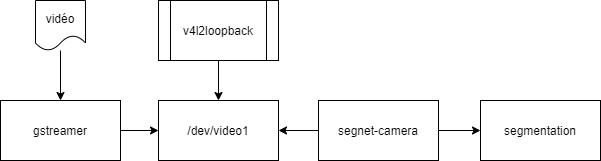
\includegraphics[width=.5\textwidth]{arch_segmentation_video}
    \caption[Diagramme d'architecture de la segmentation d'une vidéo]{Diagramme d'architecture de la segmentation d'une vidéo}
    \label{fig:arch_segmentation_video}
\end{figure}
\begin{figure}[H]
    \centering
    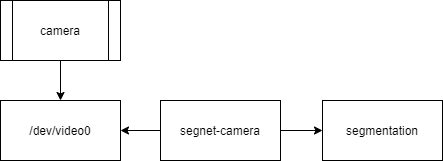
\includegraphics[width=.5\textwidth]{arch_segmentation_camera}
    \caption[Diagramme d'architecture de la segmentation avec la caméra]{Diagramme d'architecture de la segmentation avec la caméra}
    \label{fig:arch_segmentation_camera}
\end{figure}
\myparagraph{Segmentation et évaluation}
\par Les tests de performance de la segmentation de vidéos se déroulent de la manière précisée dans la section "\ref{section:strategie_test_inference} \nameref{section:strategie_test_inference}". 
\par L'un des avantages de l'utilitaire "gstreamer" est de pouvoir contrôler la résolution et le nombre d'images par seconde (\acrshort{fps}) de la vidéo qui doit être segmentée. Les différentes résolutions et \acrshort{fps} qui désirent être exécutées sont préparées dans un script "shell" écrit pour l'occasion. Le script s'occupe de démarrer gstreamer avec les bons paramètres, et en parallèle de démarrer la segmentation avec "segnet-camera". Un jeu de résolution peut être testé unitairement\footnote{\url{https://github.com/vince7lf/gae724/blob/master/run_deepscene.sh}}, ou plusieurs en séquence\footnote{\url{https://github.com/vince7lf/gae724/blob/master/run_deepscene_batch.sh}}. 
\par Les résolutions et images par seconde qui ont été testées sont résumées dans le tableau "\ref{table:resolutions_tested}". 
\par Deux vidéos ont été utilisées pour tester la segmentation. La première vidéo est utilisée pour tester l'inférence avec une vidéo du site d'étude, et qui a été fournie gracieusement par l'\acrlong{apcpontjc}. Cette première vidéo est intéressante, car elle est filmée en mouvement par un cycliste. Dans un interval de 30 secondes, l'angle de vue change rapidement. La piste cyclable est bordée d'un muret côté sud, et de la route avec les voitures qui circulent côté nord. Même si la journée est ensoleillée, la surface de la piste est aussi à un moment humide.
\par La seconde vidéo est utilisée pour tester la segmentation avec les différentes résolutions et images par seconde. C'est une vidéo d'une petite piste cyclable qui est dans mon quartier, et que j'ai prise en marchant avec mon téléphone intelligent. La vidéo est intéressante, car dans un interval de 30 secondes l'état de la piste passe d'une scène ensoleillée à ombragée, sèche à mi-sèche, avec un petit ou gros banc de neige en bordure, ou qui s'aventure un peu sur la piste, bordée d'herbe mouillée ou sèche.
\subsection{Adaptation}
\noindent La phase d'adaptation sera initiée si le temps le permet, et s'il est jugé bon d'améliorer la qualité de la segmentation. Il y a deux types d'adaptation possible: matérielle et logicielle.
\vspace{\baselineskip}
\\
\noindent L'adaptation matérielle sera jugée nécessaire si le nano ordinateur ne peut être utilisé tel quel pour répondre aux objectifs. Par exemple si le nano ordinateur devient non utilisable (lent ou sans réponse) après un certain temps. La stratégie sera de diagnostiquer le comportement et d'évaluer un remède. L'une des pistes de solution privilégiée sera de lui apporter plus de puissance, comme de l'ajout de mémoires ou un espace de stockage plus performant. Plus complexe, optimiser le processus, par exemple certains traitements, serait aussi une option.
\vspace{\baselineskip}
\\
\noindent L'adaptation logicielle, quant à elle, sera jugée nécessaire si la prédiction de la segmentation est en deçà des attentes, ou inutilisable. Le choix d'adapter un modèle avec les méthodes de "Transfer Learning" et "Domain adaptation" sera la première option privilégiée, car cela procure un gain de temps non négligeable: il n'y a pas besoin de passer à travers tout le processus "essai-erreur", couteux en temps, en énergie et en ressources matérielles, d'apprentissage et de paramétrisation du modèle. Des efforts conséquents seront par contre nécessaires pour générer les images vérités terrain \acrshort{gt} avec le jeu de données local, celui de l'\acrshort{apcpontjc} de préférence, personnel ou autre sinon.
\vspace{\baselineskip}
\\
\noindent Le diagramme de la figure \ref{fig:metho_adaptation} présente la méthodologie qu'il faut suivre pour adapter un modèle à un nouveau jeu de données et à une autre résolution. La première étape est de sélectionner un modèle déjà entrainé et qui semble pouvoir être le meilleur candidat pour aider à répondre à la problématique. C'est un travail de recherche et de test minutieux, qui est le plus important de toutes les étapes. La seconde activité est conséquente en efforts: préparer le jeu de données, incluant les images vérité terrain, les bonnes résolutions, déterminer les classes et la palette de couleurs nécessaires. L'étape suivante est d'étudier l'architecture du modèle, afin de l'adapter au jeu de données, aux classes, et au besoin modifier les couches de l'architecture afin d'avoir une segmentation la plus précise et fine possible. Une fois ces étapes de préparation complétées, le ré entrainement du modèle peut s'effectuer, et la segmentation évaluée. Cette phase d'adaptation est un processus itératif, qui peut être représenté par la figure \ref{fig:methodologie_complexe_realiste}.
\label{metho_adaptation}
\begin{figure}[H]
    \centering
    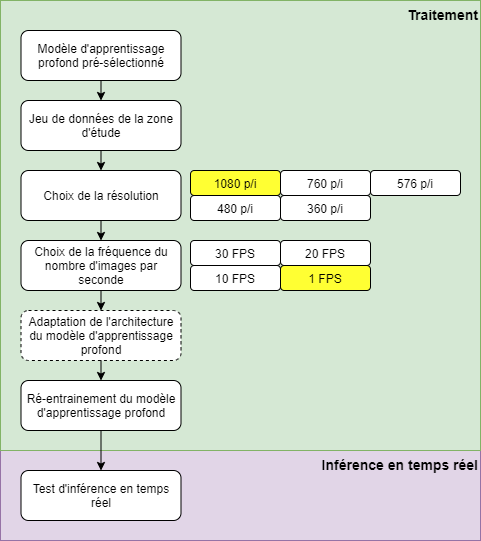
\includegraphics[width=0.65\textwidth]{metho_traitement_eval.png}
    \caption{Méthodologie du traitement et adaptation}
    \label{fig:metho_adaptation}
\end{figure}
\subsubsection{Choix du modèle de l'architecture FCN}
\noindent Le premier modèle qui est évalué est celui de l'architecture SegNet18 entrainée avec le jeu de données "DeepSCene", et fourni par NVIDIA. Le second de la liste, et qui est aussi déjà fourni par NVIDIA, est l'architecture de SegNet18 entrainée avec le jeu de donnée "CityScape". Les deux autres architectures, ResNet101 \& DeepScene et DeepLabV3 \& Deepscene, ne sont pas disponibles et devront être préparées et entrainées, mais elles sont attrayantes du point de vue de leur réputation et de leur potentiel, et vouloir les adapter au contexte de l'essai semble logique. Une dernière boite vide est disponible, afin de laisser une porte ouverte à une potentielle opportunité d'entrainer une architecture tout à fait personnalisée, par exemple une adaptation de l'architecture de DeepLabV3 avec le jeu de données de l'\acrshort{apcpontjc}.
\subsubsection{Adaptation du modèle}
% {\color{red}\todo{TODO}}
\subsubsection{Ré-entrainement du modèle}
% {\color{red}\todo{TODO}}